\documentclass{beamer-custom}
\usepackage{beamer-custom}

\usefonttheme{serif}
% Theme
\usetheme{Montpellier}
\usecolortheme{beaver}
\useinnertheme{circles}

% Navigation
\setbeamertemplate{navigation symbols}{}
\setbeamertemplate{footline}[frame number]

% Frame title formatting
\setbeamertemplate{frametitle}{
    \vspace{0.5em}
    \insertframetitle
    \par
}
%\usepackage{cmbright,bbold}
%\renewcommand{\mathcal}{\mathtt}
\usepackage{kpfonts}
\AtBeginSection[]
{
  \begin{frame}
    \frametitle{Contents}
    \tableofcontents[currentsection]
  \end{frame}
}
% Title page
\title{Amenability: A (Somewhat) Brief Introduction}
\author{Avinash Iyer}
\institute{Occidental College}
\date{March 20, 2025}
\DeclareMathOperator{\op}{op}

\begin{document}
\begin{frame}
    \titlepage
\end{frame}

\begin{frame}{Outline}
    \tableofcontents
\end{frame}
\section{Definitions}%
\begin{frame}
  \frametitle{Groups}
  If $A$ is a set, and $\star\colon A\times A \rightarrow A$ is an operation such that
  \begin{itemize}
    \item $a\star\left(b\star c\right) = \left(a\star b\right)\star c$;
    \item there exists $e_A$ such that $a\star e_A = e_A\star a = a$;
    \item for each $a$ there exists $a^{-1}$ such that $a\star a^{-1} = a^{-1}\star a = e_A$,
  \end{itemize}
  then we call the pair $\left(A,\star\right)$ a \textit{group}.\pause\hfill\break

  We abbreviate $a\star b$ as $ab$. If $ab = ba$, then we say the group is \textit{abelian}.
\end{frame}
\begin{frame}
  \frametitle{Subgroups, Quotient Groups}
  Let $G$ be a group.
  \begin{itemize}
    \item If $H\subseteq G$ is a subset that satisfies, for all $a,b\in H$, $ab^{-1}\in H$, then we say $H$ is a \textit{subgroup}.\pause
    \item If $N\subseteq G$ is a subgroup that satisfies, for all $g\in G$ and $h\in N$, $ghg^{-1}\in N$, then we say $N$ is a \textit{normal subgroup}.\pause
    \item The equivalence classes under the relation $g\sim_{N} g'$ if $g^{-1}g' \in N$ form a group $gN\coloneqq \left[ g \right]_{\sim}$ known as the \textit{quotient group} $G/N$.
    \item The \textit{index} of a subgroup $H\leq G$ is the number of cosets, $gH\coloneqq \set{gh | h\in H}$, written $\left[ G:H \right]$.
  \end{itemize}
\end{frame}
\begin{frame}
  \frametitle{Some Groups}
  \begin{itemize}
    \item The integers $\Z$ are a group under addition.
    \item The group of invertible $n\times n$ matrices over $\C$, $\text{GL}_{n}\left(\C\right)$, is a group under matrix multiplication.
    \item The subgroup $\text{SO}(n)\subseteq \text{GL}_{n}\left( \R \right)$ consisting of $n\times n$ orthogonal matrices with determinant $1$ is a group under multiplication.
  \end{itemize}
\end{frame}
\begin{frame}
  \frametitle{Group Actions}
  Let $G$ be a group, and $X$ a set. Let $\rho\colon G\times X \rightarrow X$ be a function that satisfies, for all $g,h\in G$ and $x\in X$,
  \begin{itemize}
    \item $\rho\left( e_G, x\right) = x$;
    \item $\rho\left( g,\rho\left( h,x \right) \right) = \rho\left( gh,x \right)$.
  \end{itemize}
  Then, we say $\rho$ is an \textit{action} of $G$ on $X$. We write $\rho\left( g,x \right) = g\cdot x$.
\end{frame}
\begin{frame}
  \frametitle{$\sigma$-Algebras and Measures}
  If $X$ is a set, then a collection of subsets $\set{A_{i}}_{i\in I} = \mathcal{A}\subseteq P(X)$ is known as an \textit{algebra} of subsets if
  \begin{enumerate}
    \item $\emptyset,X\in \mathcal{A}$;
    \item for any $A_i\in \mathcal{A}$, $A_i^{c}\in \mathcal{A}$;
    \item for any $A_i,A_j\in \mathcal{A}$, $A_i\cup A_j\in \mathcal{A}$.
  \end{enumerate}\pause
  If, for any countable collection, $\set{A_n}_{n\geq 1}\subseteq \mathcal{A}$, condition (3) holds, then we say $\mathcal{A}$ is a \textit{$\sigma$-algebra} of subsets.
\end{frame}
\begin{frame}
  \frametitle{$\sigma$-Algebras and Measures, Cont'd}
  If $X$ is a set and $\mathcal{A}$ is a $\sigma$-algebra, then a map $\mu\colon \mathcal{A}\rightarrow [0,\infty]$ that satisfies:
  \begin{itemize}
    \item $\mu\left( \emptyset \right) = 0$;
    \item for disjoint sets $A,B\in \mathcal{A}$, $\mu\left( A\sqcup B \right) = \mu\left( A \right) + \mu\left( B \right)$,
  \end{itemize}
  then we say $\mu$ is a \textit{finitely additive} measure.\pause \newline

  If $\set{A_n}_{n\geq 1}$ is a countable collection of disjoint sets, then if $\mu$ satisfies
  \begin{itemize}
    \item $\displaystyle \mu\left( \bigcup_{n\geq 1}A_n \right) = \sum_{n\geq 1}\mu\left( A_n \right)$,
  \end{itemize}
  we say $\mu$ is a measure. If $\mu\left( X \right) = 1$, then we say $\mu$ is a probability measure.
\end{frame}
\section{Paradoxical Decompositions}%
\begin{frame}
  \frametitle{Questions?}
  \begin{itemize}
    \item If $G$ is a group, is it possible to reconstruct $G$ by using some subset of $G$?
    \item When may we find a finitely additive probability measure $\mu\colon P(G)\rightarrow [0,1]$ such that $\mu\left( E \right) = \mu\left( tE \right)$ for all $E\subseteq G$?
    \item Are these questions even related?
  \end{itemize}
\end{frame}
\begin{frame}
  \frametitle{Free Groups}
  \begin{itemize}
    \item We begin by considering a special group, known as $F(a,b)$ or the \textit{free group on two generators}.\pause
    \item We define $F(a,b)$ to be the set of all ``words'' in the alphabet $\set{a,b,a^{-1},b^{-1}}$, subject to the condition that, for $w,w'\in F(a,b)$,
      \begin{align*}
        waa^{-1}w' \sim wa^{-1}aw' \sim ww'\\
        wbb^{-1}w' \sim wb^{-1}bw' \sim ww'.
      \end{align*}
    \item Examples: $a^2bab^{-1},b^{-1}a^2b^2ab\in F(a,b)$.
  \end{itemize}
\end{frame}
\begin{frame}
  \frametitle{A Curiosity}
  Let $W(b)\subseteq F(a,b)$ be all the words that start with $b$. Then, $b^{-1}W(b)$ consists of \pause
  \begin{itemize}
    \item all words that start with $a$;
    \item all words that start with $a^{-1}$;
    \item all words that start with $b$ --- think words that start with $b^2$ before you multiply $b^{-1}$.\pause
  \end{itemize}
  Thus, all we need to do is add back $W\left( b^{-1} \right)$ to get $F(a,b)$ back.
  \begin{align*}
    F(a,b) &= W\left( b^{-1} \right)\cup b^{-1}W(b).
  \end{align*}
\end{frame}
\begin{frame}
  \frametitle{A Curiosity, Cont'd}
  Similarly, we can do this for $a$, giving a decomposition of $F(a,b)$ in two separate ways:
  \begin{align*}
    F(a,b) &= b^{-1}W(b)\cup W\left( b^{-1} \right)\\
           &= a^{-1}W(a)\cup W\left( a^{-1} \right).
  \end{align*}\pause
  Furthermore, note that $W\left( a \right),W\left( b \right),W\left( a^{-1} \right),W\left( b^{-1} \right)$ are disjoint.\pause\newline

  We're able to take part of the group $F(a,b)$, take some translations, and, miraculously, obtain the entire group back.
\end{frame}
\begin{frame}
  \frametitle{Defining Paradoxical Decompositions}
  Let $G$ be a group. A \textit{paradoxical decomposition} of $G$ consists of
  \begin{itemize}
    \item pairwise disjoint subsets $A_1,\dots,A_n,B_1,\dots,B_m\subseteq G$; and
    \item elements $g_1,\dots,g_n,h_1,\dots,h_m\in G$;
  \end{itemize}
  such that
  \begin{align*}
    G &= \bigcup_{i=1}^{n}g_iA_i\\
      &= \bigcup_{j=1}^{m}h_jB_j.
  \end{align*}\pause
  If $G$ admits a paradoxical decomposition, we say $G$ is \textit{paradoxical}.
\end{frame}
\begin{frame}
  \frametitle{Paradoxical Actions}
  If $G$ acts on a set $X$, then a subset $A\subseteq X$ is \textit{$G$-paradoxical} if there exist
  \begin{itemize}
    \item pairwise disjoint subsets $A_1,\dots,A_n,B_1,\dots,B_m\subseteq A$; and
    \item elements $g_1,\dots,g_n,h_1,\dots,h_m\in G$
  \end{itemize}
  such that
  \begin{align*}
    A &= \bigcup_{i=1}^{n}g_i\cdot A_i\\
      &= \bigcup_{j=1}^{m}h_j\cdot B_j.
  \end{align*}\pause
  A paradoxical group is a paradoxical set under the action of left-multiplication.
\end{frame}
\begin{frame}
  \frametitle{Depiction}
%  \begin{center}
%    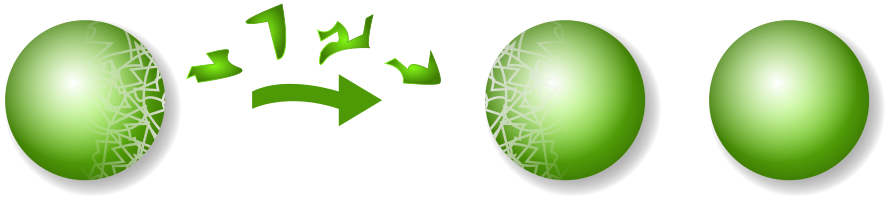
\includegraphics[scale=0.17]{images/paradoxical_decomposition_3.png}
%  \end{center}
  \begin{center}
\tikzset{every picture/.style={line width=0.75pt}} %set default line width to 0.75pt        

\begin{tikzpicture}[x=0.75pt,y=0.75pt,yscale=-1,xscale=1,scale=0.5]
%uncomment if require: \path (0,463); %set diagram left start at 0, and has height of 463

%Shape: Circle [id:dp7888194146123797] 
\draw   (181,100.5) .. controls (181,57.15) and (216.15,22) .. (259.5,22) .. controls (302.85,22) and (338,57.15) .. (338,100.5) .. controls (338,143.85) and (302.85,179) .. (259.5,179) .. controls (216.15,179) and (181,143.85) .. (181,100.5) -- cycle ;
%Shape: Circle [id:dp617800520698538] 
\draw   (442,105.5) .. controls (442,62.15) and (477.15,27) .. (520.5,27) .. controls (563.85,27) and (599,62.15) .. (599,105.5) .. controls (599,148.85) and (563.85,184) .. (520.5,184) .. controls (477.15,184) and (442,148.85) .. (442,105.5) -- cycle ;
%Shape: Circle [id:dp7464117940471128] 
\draw   (323,316.5) .. controls (323,273.15) and (358.15,238) .. (401.5,238) .. controls (444.85,238) and (480,273.15) .. (480,316.5) .. controls (480,359.85) and (444.85,395) .. (401.5,395) .. controls (358.15,395) and (323,359.85) .. (323,316.5) -- cycle ;
%Curve Lines [id:da5554211938824235] 
\draw [line width=0.75] [line join = round][line cap = round]   (291,173) .. controls (291,159.08) and (283.63,146.13) .. (279,133) .. controls (271.16,110.79) and (278.88,78.12) .. (295,62) .. controls (300.41,56.59) and (306.47,45) .. (313,45) ;
%Curve Lines [id:da08915852048267425] 
\draw [line width=0.75] [line join = round][line cap = round]   (209.39,161.59) .. controls (209.39,130.53) and (249.15,131.7) .. (270.89,132.41) .. controls (274.41,132.52) and (277.64,135.65) .. (280.61,135.65) ;
%Curve Lines [id:da035853299183386755] 
\draw [line width=0.75] [line join = round][line cap = round]   (260,22) .. controls (260,26.67) and (259.34,31.38) .. (260,36) .. controls (261.29,45.01) and (280.44,69) .. (289,69) ;
%Curve Lines [id:da3831843525173042] 
\draw [line width=0.75] [line join = round][line cap = round]   (220.28,32.86) .. controls (220.28,52.33) and (233.93,70.2) .. (223.48,89.3) .. controls (220.12,95.42) and (216.8,104.42) .. (213.89,109.73) .. controls (211.59,113.94) and (203.25,119.45) .. (200.04,122.38) .. controls (197.37,124.82) and (188.33,128.76) .. (188.33,131.14) ;
%Curve Lines [id:da08149494112624311] 
\draw    (188,105) .. controls (89.49,217.44) and (273.15,339.77) .. (338.03,365.62) ;
\draw [shift={(339,366)}, rotate = 201.34] [color={rgb, 255:red, 0; green, 0; blue, 0 }  ][line width=0.75]    (10.93,-3.29) .. controls (6.95,-1.4) and (3.31,-0.3) .. (0,0) .. controls (3.31,0.3) and (6.95,1.4) .. (10.93,3.29)   ;
%Curve Lines [id:da8168391395626808] 
\draw    (236,163) .. controls (201.35,212.5) and (301.95,255.14) .. (347.63,256.96) ;
\draw [shift={(349,257)}, rotate = 181.27] [color={rgb, 255:red, 0; green, 0; blue, 0 }  ][line width=0.75]    (10.93,-3.29) .. controls (6.95,-1.4) and (3.31,-0.3) .. (0,0) .. controls (3.31,0.3) and (6.95,1.4) .. (10.93,3.29)   ;
%Curve Lines [id:da9056524070522074] 
\draw    (209,132) .. controls (165.44,212.19) and (275.76,298.26) .. (321.63,309.68) ;
\draw [shift={(323,310)}, rotate = 192.53] [color={rgb, 255:red, 0; green, 0; blue, 0 }  ][line width=0.75]    (10.93,-3.29) .. controls (6.95,-1.4) and (3.31,-0.3) .. (0,0) .. controls (3.31,0.3) and (6.95,1.4) .. (10.93,3.29)   ;
%Curve Lines [id:da22269351080305821] 
\draw    (320,135) .. controls (333.86,203.31) and (423.19,198.11) .. (463.78,168.89) ;
\draw [shift={(465,168)}, rotate = 143.13] [color={rgb, 255:red, 0; green, 0; blue, 0 }  ][line width=0.75]    (10.93,-3.29) .. controls (6.95,-1.4) and (3.31,-0.3) .. (0,0) .. controls (3.31,0.3) and (6.95,1.4) .. (10.93,3.29)   ;
%Curve Lines [id:da5779701148660346] 
\draw    (285,33) .. controls (324.4,3.45) and (448.21,20.47) .. (491.1,27.68) ;
\draw [shift={(493,28)}, rotate = 189.69] [color={rgb, 255:red, 0; green, 0; blue, 0 }  ][line width=0.75]    (10.93,-3.29) .. controls (6.95,-1.4) and (3.31,-0.3) .. (0,0) .. controls (3.31,0.3) and (6.95,1.4) .. (10.93,3.29)   ;

% Text Node
\draw (302,94) node [anchor=north west][inner sep=0.75pt]   [align=left] {\tiny$ A_{1}$};
% Text Node
\draw (273,33) node [anchor=north west][inner sep=0.75pt]   [align=left] {\tiny$ A_{2}$};
% Text Node
\draw (241,145) node [anchor=north west][inner sep=0.75pt]   [align=left] {\tiny $ B_{1}$};
% Text Node
\draw (239,75) node [anchor=north west][inner sep=0.75pt]   [align=left] {\tiny $ B_{2}$};
% Text Node
\draw (191,73) node [anchor=north west][inner sep=0.75pt]   [align=left] {\tiny$ B_{3}$};
% Text Node
\draw (188,287) node [anchor=north west][inner sep=0.75pt]   [align=left] {\small $ h_{3}$};
% Text Node
\draw (241,238) node [anchor=north west][inner sep=0.75pt]   [align=left] {\small$ h_{2}$};
% Text Node
\draw (260,204) node [anchor=north west][inner sep=0.75pt]   [align=left] {\small$ h_{1}$};
% Text Node
\draw (381,161) node [anchor=north west][inner sep=0.75pt]   [align=left] {\small$ g_{1}$};
% Text Node
\draw (400,19) node [anchor=north west][inner sep=0.75pt]   [align=left] {\small $ g_{2}$};


\end{tikzpicture}
  \end{center}
\end{frame}
\begin{frame}
  \frametitle{Examples}
  \begin{itemize}
    \item The free group $F(a,b)$ is paradoxical.\pause
    \item Any group that contains a paradoxical subgroup is paradoxical.
    \item $F(S)$, where $S$ is any nonempty set with more than two elements, is paradoxical.
  \end{itemize}
\end{frame}
\begin{frame}
  \frametitle{A Paradoxical Subgroup of $\text{SO}(3)$}
  The following two matrices (and their inverses) generate a subgroup of $\text{SO}(3)$ that is isomorphic to $F(a,b)$.
  \begin{align*}
    A &= \begin{pmatrix}3/5 & 4/5 & 0 \\  -4/5 & 3/5 & 0 \\ 0 & 0 & 1\end{pmatrix}\\
    B &= \begin{pmatrix}1 & 0 & 0 \\ 0 & 3/5 & -4/5 \\ 0 & 4/5 & 3/5\end{pmatrix}.
  \end{align*}\pause
  This is proven using the Ping-Pong lemma.
\end{frame}
\begin{frame}
  \frametitle{Introducing the Banach--Tarski Paradox}
  \begin{theorem}[The Banach--Tarski Paradox]
    Let $A$ and $B$ be bounded subsets of $\R^3$ with nonempty interior. There is a partition of $A$ into finitely many disjoint subsets such that a sequence of isometries applied to these subsets yields $B$.
  \end{theorem}\pause
  \begin{itemize}
    \item In other words, not all subsets of $\R^3$ have a definite ``volume'' invariant under isometry.
  \end{itemize}
\end{frame}
\begin{frame}
  \frametitle{Equidecomposability}
  Let $G$ be a group that acts on a set $X$, and let $A,B\subseteq X$. If there exist
  \begin{itemize}
    \item finite partitions, $A_1,\dots,A_n\subseteq A$, $B_1,\dots,B_n\subseteq B$
    \item group elements $g_1,\dots,g_n\in G$
  \end{itemize}
  such that $g_i\cdot A_i = B_i$, then we say $A$ and $B$ are \textit{$G$-equidecomposable}.\pause\newline

  Effectively, $A$ and $B$ are ``equal'' to each other up to the group action.\pause\newline

  If $A$ is $G$-paradoxical, then so too is $B$.
\end{frame}
\begin{frame}[allowframebreaks]
  \frametitle{The Banach--Tarski Paradox: Proof Outline}
  \begin{enumerate}[(1)]
    \item We use the two matrices
      \begin{align*}
        A &= \begin{pmatrix}3/5 & 4/5 & 0 \\  -4/5 & 3/5 & 0 \\ 0 & 0 & 1\end{pmatrix}\\
        B &= \begin{pmatrix}1 & 0 & 0 \\ 0 & 3/5 & -4/5 \\ 0 & 4/5 & 3/5\end{pmatrix}.
      \end{align*}
      to generate a subgroup of $\text{SO}\left( 3 \right)$ isomorphic to $F(a,b)$.
    \item We use the decomposition 
      \begin{align*}
        F\left( a,b \right) &= a^{-1}W\left( a \right)\cup W\left( a^{-1} \right)\\
                            &= b^{-1}W\left( b \right) \cup W\left( b^{-1} \right)
      \end{align*}
      to duplicate the unit sphere in $\R^3$, $S^2$, except for a countable subset $D$. (The \textit{Hausdorff Paradox}.)
    \item We show that $S^2$ and $S^2\setminus D$ are $\text{SO}\left( 3 \right)$-equidecomposable --- there is thus a paradoxical decomposition of $S^2$.
    \item We show that the unit ball, $B\left( 0,1 \right)\subseteq \R^3$, is paradoxical under the isometry group $\text{E}\left( 3 \right)$.
    \item Define a relation $A\preceq B$ if $A$ is $G$-equidecomposable with a subset of $B$, and show that if $A\preceq B$ and $B\preceq A$, then $A$ and $B$ are $G$-equidecomposable.
    \item Show that $A\subseteq \R^3$ is equidecomposable with a subset of $B\subseteq \R^3$.\pause
  \end{enumerate}
  We're done...\pause or are we?
\end{frame}
\section{From Paradoxical Decompositions to Amenability}%
\begin{frame}
  \frametitle{Ill-Behaved Groups}
  \begin{itemize}
    \item The way that our copy of $F(a,b)$ helped ``create'' the Banach--Tarski paradox suggests that $F(a,b)$ is a particularly ill-behaved group.
    \item Let $\nu\colon F(a,b)\rightarrow [0,1]$ be a probability measure --- we will show that $\nu$ \textit{cannot} be translation-invariant (i.e., $\nu\left( tE \right) = \nu\left( E \right)$ for all $t\in F(a,b),E\subseteq F(a,b)$).
  \end{itemize}
\end{frame}
\begin{frame}
  \frametitle{Ill-Behaved Groups, Cont'd}
  Suppose such a translation-invariant $\nu$ exists. Taking
  \begin{align*}
    F(a,b) &= W(a)\sqcup W\left( a^{-1} \right) \sqcup W\left( b \right) \sqcup W\left( b^{-1} \right),
  \end{align*}
  we have
  \begin{align*}
    1 &= \nu\left( W\left( a \right) \right) + \nu\left( W\left( a^{-1} \right) \right) + \nu\left( W\left( b \right) \right) + \nu\left( W\left( b^{-1} \right) \right)\\
      &= \nu\left( a^{-1}W\left( a \right) \right) + \nu\left( W\left( a^{-1} \right) \right) + \nu\left( b^{-1}W\left( b \right) \right) + \nu\left( W\left( b^{-1} \right) \right)\\
      &= \nu\left( a^{-1}W\left( a \right)\sqcup W\left( a^{-1} \right) \right) + \nu\left( b^{-1}W\left( b \right) \sqcup W\left( b^{-1} \right) \right)\\
      &= \nu\left( F(a,b) \right) + \nu\left( F(a,b) \right)\\
      &= 2.
  \end{align*}\pause
  Huh.
\end{frame}
\begin{frame}
  \frametitle{Amenability}
  Let $G$ be a group. A \textit{mean} is a finitely additive probability measure $\nu\colon G\rightarrow [0,1]$ such that
  \begin{align*}
    \nu\left( tE \right) &= \nu\left( E \right)
  \end{align*}
  for all $t\in G$ and $E\subseteq G$.\newline

  If $G$ admits a mean, we say $G$ is \textit{amenable}.\pause
  \begin{itemize}
    \item In other words, $G$ is sufficiently ``well-behaved.''
  \end{itemize}
\end{frame}
\begin{frame}
  \frametitle{Inheritance Properties of Amenability}
  \begin{itemize}
    \item If $G$ is amenable, then any subgroup of $G$ is amenable.
    \item If $G$ is amenable, then quotient groups, $G/N$, are amenable.
    \item If $H\leq G$ is an amenable subgroup such that $\left[ G:H \right] < \infty$, then $G$ is amenable.
    \item If $N\trianglelefteq G$ and $G/N$ are amenable, then $G$ is amenable.
    \item If $\left( G_i,\varphi_i \right)_{i\in I}$ is a directed system of amenable groups, then the union $G = \bigcup_{i\in I}G_i$ is amenable.
  \end{itemize}
\end{frame}
\begin{frame}
  \frametitle{Examples}
  \begin{itemize}
    \item Finite groups are amenable: let $\delta_t$ be the point mass at $t\in G$,
      \begin{align*}
        \delta_t(s) &= \begin{cases}
          1 & t = s\\
          0 & t\neq s
        \end{cases}.
      \end{align*}
      Then,
      \begin{align*}
        \nu &= \frac{1}{\left\vert G \right\vert} \sum_{t\in G}\delta_t
      \end{align*}
      is a mean.
    \item Abelian groups are amenable.
    \item The free group, $F(a,b)$, is \textit{not} amenable.
  \end{itemize}
\end{frame}
\begin{frame}
  \frametitle{Paradoxical Groups and Amenability}
  Every paradoxical group is \textit{not} amenable --- the argument is similar to the case for $F(a,b)$.\pause\newline

  More surprisingly, though, every \textit{non}-paradoxical group is amenable.\pause
  \begin{theorem}[Tarski's Theorem]
    Let $G$ be a group. Then, $G$ is non-paradoxical if and only if $G$ is amenable.
  \end{theorem}\pause
  Unfortunately, the proof that every non-paradoxical group is amenable is significantly harder.
\end{frame}
\section{Equivalent Definitions and Other Criteria}%
% Følner condition, Cayley graph, talk about intuition behind Følner condition
% Growth, Functional Analysis, Representations, 
\begin{frame}
  \frametitle{Why Find Alternative Characterizations?}
  On first glance, it may seem like we're finished, but we're really not.\pause\newline

  Our methods so far --- the existence of a mean, or showing non-paradoxicality --- are quite difficult to establish.\pause\newline

  As it turns out, amenability touches a variety of fields:
  \begin{itemize}
    \item functional analysis;
    \item geometric group theory;
    \item representation theory;
    \item operator algebras.
  \end{itemize}
\end{frame}
\subsection{A Taste of Functional Analysis}%
\begin{frame}
  \frametitle{Function Spaces}
  Functions are much easier to work with than sets and measures (or at least, they're more interesting to work with).\pause\newline

  We work with three special function spaces over the group $\Gamma$.
  \begin{align*}
    \ell_{\infty}\left( \Gamma \right) &\coloneqq \set{f\colon \Gamma\rightarrow \C | \sup_{t\in\Gamma}\left\vert f(t) \right\vert < \infty};\\
    \ell_{1}\left( \Gamma \right) &\coloneqq \set{f\colon \Gamma\rightarrow \C | \sum_{t\in\Gamma}\left\vert f(t) \right\vert < \infty};\\
    \ell_{2}\left( \Gamma \right) &\coloneqq \set{f\colon \Gamma\rightarrow \C | \sum_{t\in\Gamma}\left\vert f(t) \right\vert^2 < \infty}.
  \end{align*}
\end{frame}
\begin{frame}
  \frametitle{Work in $\ell_{\infty}(\Gamma)$}
  For a given $f\in\ell_{\infty}\left( \Gamma \right)$, we define
  \begin{align*}
    \lambda_s\colon \ell_{\infty}\left( \Gamma \right)\rightarrow \ell_{\infty}\left( \Gamma \right)
  \end{align*}
  by $\lambda_s\left( f \right)\left( t \right) = f\left( s^{-1}t \right)$.\pause\newline

  If there is some $\rho\colon \ell_{\infty}\left( \Gamma \right)\rightarrow \C$ such that
  \begin{itemize}
    \item $\rho\left( \1_{\Gamma} \right) = 1 = \norm{\rho}_{\op}$;
    \item $\rho\left( f \right) = \rho\left( \lambda_s(f) \right)$,
  \end{itemize}
  then we call $\rho$ an \textit{invariant state}.
\end{frame}
\begin{frame}
  \frametitle{Work in $\ell_{\infty}\left( \Gamma \right)$, cont'd}
  Invariant states and means are interchangeable.\pause\newline

  Define
  \begin{align*}
    \mu\left( E \right) &= \rho\left( \1_{E} \right)
  \end{align*}
  for all $E\subseteq \Gamma$.
\end{frame}
\subsection{Introducing Approximations}%
\begin{frame}
  \frametitle{Motivating Følner's Condition}
  There is actually one way that working with sets makes life easier.\pause\newline

  Remember when we decomposed
  \begin{align*}
    F(a,b) &= W(a) \sqcup W\left( a^{-1} \right) \sqcup W\left( b \right) \sqcup W\left( b^{-1} \right).
  \end{align*}
  Translating $W\left( a \right) \mapsto a^{-1}W\left( a \right)$ gave us a set that was ``significantly'' ``bigger'' than $W\left( a^{-1} \right)$; specifically, it gave us $F\left( a,b \right) \setminus W\left( a^{-1} \right)$.
\end{frame}
\begin{frame}
  \frametitle{Følner's Condition}
  We can actually make this sense of ``bigness'' precise --- if the symmetric difference of the translated set and our original set becomes ``sufficiently small,'' then we can put a mean on the group.\pause
  \begin{theorem}[Følner's Theorem]
    Let $\Gamma$ be a (countable, discrete) group. Then, $\Gamma$ is amenable if and only if there exists a sequence $\left( F_n \right)_n$ of finite sets such that for all $s\in \Gamma$,
    \begin{align*}
      \lim_{n\rightarrow\infty}\frac{\left\vert sF_n\triangle F_n \right\vert}{\left\vert F_n \right\vert} &= 0.
    \end{align*}
  \end{theorem}
\end{frame}
\begin{frame}
  \frametitle{Approximating Means}
  The Følner condition allows us to find an ``approximate'' version of a mean that works in $\ell_1\left( \Gamma \right)$ instead of $\ell_{\infty}\left( \Gamma \right)$.\pause\newline

  Keeping $\lambda_s(f)(t) = f\left( s^{-1}t \right)$, we say $\left( f_k \right)_k\subseteq \ell_1\left( \Gamma \right)$ is an \textit{approximate mean} if
  \begin{align*}
    \lim_{k\rightarrow\infty}\norm{f_k - \lambda_s\left( f_k \right)}_{\ell_1} &= 0.
  \end{align*}
  \end{frame}
  \begin{frame}
  \frametitle{Approximating Means, Cont'd}
  This is equal to Følner's condition; in one direction by defining
  \begin{align*}
    f_k &= \frac{1}{\left\vert F_k \right\vert}\1_{F_k},
  \end{align*}\pause
  and in the other direction by using the ``layer cake'' decomposition
  \begin{align*}
    f &= \sum_{i=1}^{n} c_i \1_{F_i},
  \end{align*}
  where $F_1\supseteq F_2\supseteq \cdots \supseteq F_n$.
\end{frame}
\begin{frame}
  \frametitle{Using Følner's Condition}
  If $S$ is a (finite) generating set for $G$, then letting
  \begin{align*}
    S^n &\coloneq \set{g_1\cdots g_n | g_i\in S},
  \end{align*}
  we call groups such that
  \begin{align*}
    \limsup_{n\rightarrow\infty} \left\vert S^n \right\vert^{1/n} &= 1
  \end{align*}
  \textit{groups of subexponential growth}. Følner's condition is used to show that they are amenable.
\end{frame}
\begin{frame}
  \frametitle{Graphs and Amenability}
  Given a group with generating set $S$, we may define a graph --- known as the Cayley graph --- by ``walking'' along the direction that leads us to an element of the group.
  \begin{center}
    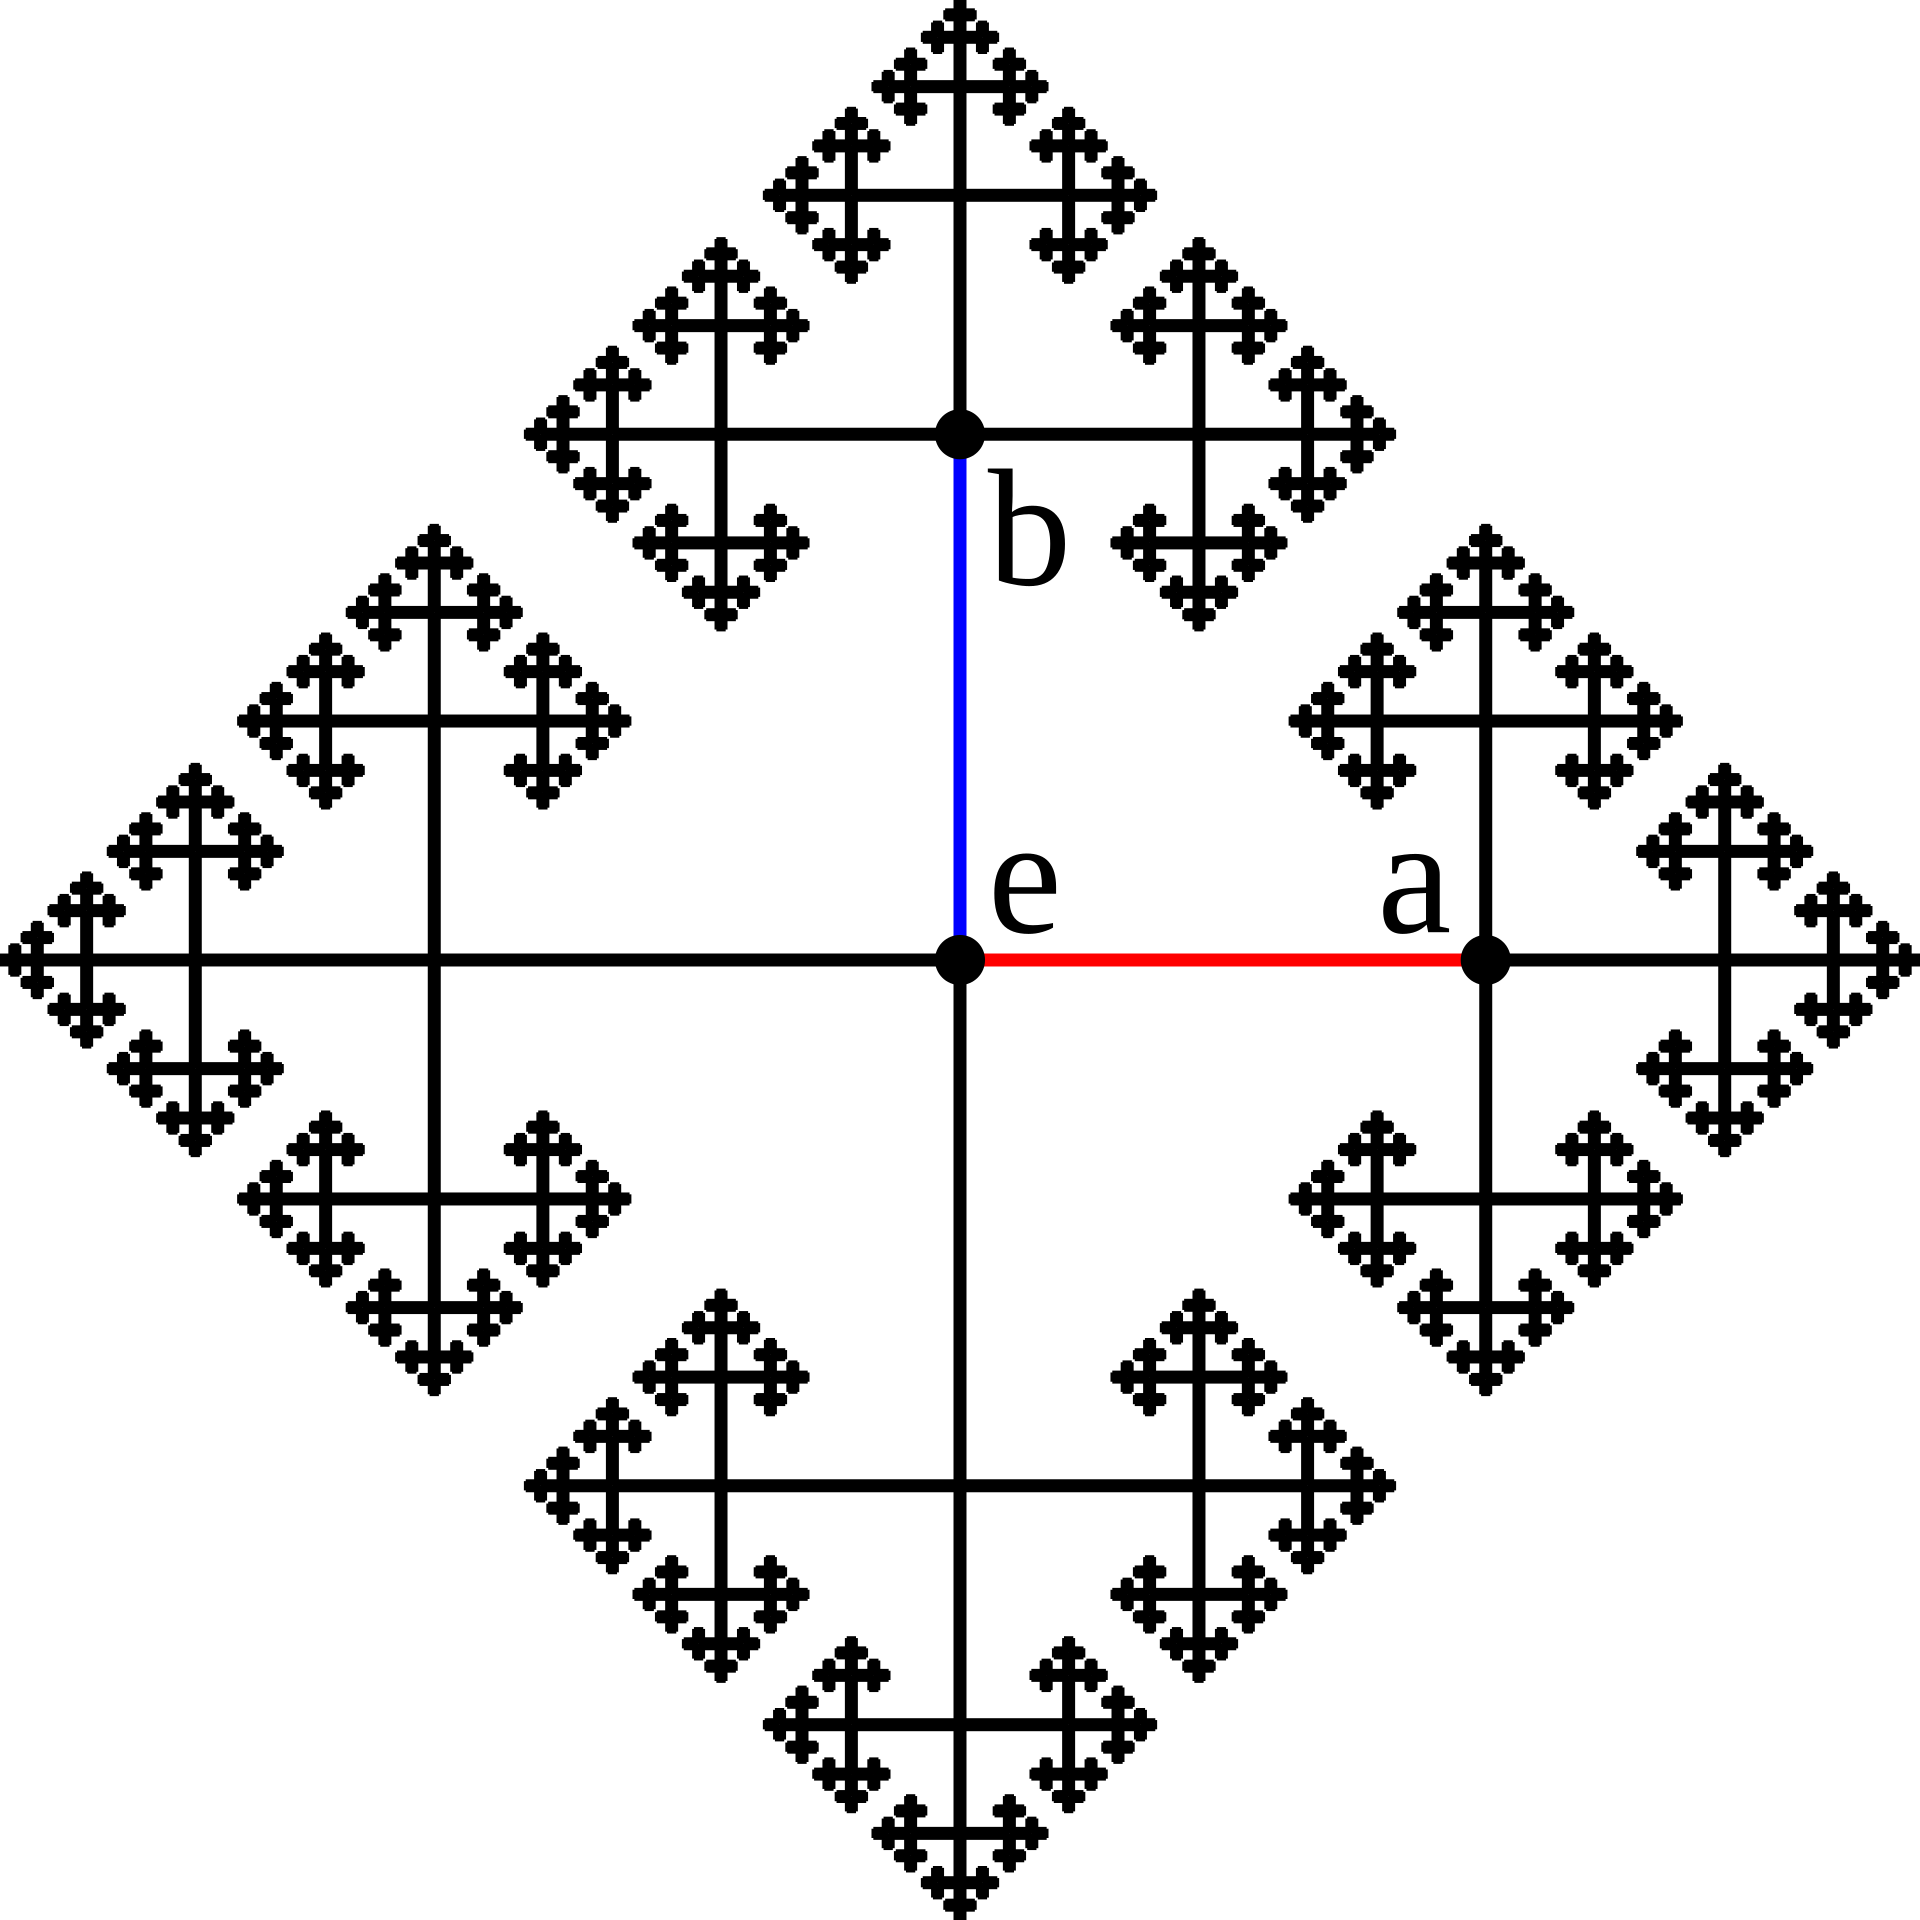
\includegraphics[scale=0.075]{images/cayley_graph.png}
  \end{center}
\end{frame}
\begin{frame}
  \frametitle{Graphs and Amenability, cont'd}
  If the Cayley graph of $G$ has a ``sufficiently slow-growing'' neighbor vertex set, then $G$ is amenable --- this is once again proven using the Følner condition.
\end{frame}
\subsection{Approximations with Representations and Operators}%
\begin{frame}
  \frametitle{Introducing the Left-Regular Representation}
  Consider the map $s \mapsto \lambda_s$, where once again $\lambda_s(f)(t) = f\left( s^{-1}t \right)$, this time when $f\in \ell_2\left( \Gamma \right)$.\pause\newline

  Then, if
  \begin{align*}
    \iprod{f}{g} &= \sum_{t\in\Gamma}f(t)\overline{g(t)},
  \end{align*}
  on $\ell_2\left( \Gamma \right)$, we have, for all $s\in\Gamma$
  \begin{align*}
    \iprod{\lambda_s(f)}{\lambda_s(g)} &= \iprod{f}{g},\\
    \lambda_s\lambda_s^{\ast} &= I\\
    \lambda_s^{\ast}\lambda_s &= I
  \end{align*}\pause
  This makes $\lambda_s$ a \textit{unitary operator} on $\ell_2\left( \Gamma \right)$ --- $\lambda_s\in \mathcal{U}\left( \ell_2\left( \Gamma \right) \right)$.
\end{frame}
\begin{frame}
  \frametitle{Introducing the Left-Regular Representation, cont'd}
  The map $s\mapsto \lambda_s$ is a group homomorphism that represents $\Gamma$ as a unitary operator on $\ell_2\left( \Gamma \right)$, known as the \textit{left-regular representation}.\pause\newline

  Unitary representations like the left-regular representation are incredibly useful.
\end{frame}
\begin{frame}
  \frametitle{The Left-Regular Representation and Amenability}
  A sequence $\left( f_k \right)_k\subseteq \ell_2\left( \Gamma \right)$ is known as an \textit{almost-invariant vector} if
  \begin{align*}
    \lim_{k\rightarrow\infty}\norm{f_k - \lambda_s\left( f_k \right)}_{\ell_2} &= 0.
  \end{align*}\pause
  This looks very similar to the approximate mean --- and its equivalence with amenability is proven using approximate means.
\end{frame}
\begin{frame}
  \frametitle{Our First $C^{\ast}$-Algebra}
  If $\Gamma$ is a group, we may define a vector space, $\C\left[ \Gamma \right]$, by finite sums
  \begin{align*}
    x &= \sum_{t\in\Gamma}x(t)\delta_t,
  \end{align*}
  where $\delta_t$ is the point mass at $t\in \Gamma$.\pause\newline

  This becomes a $\ast$-algebra when endowed with multiplication and involution:
  \begin{align*}
    f\ast g(s) &= \sum_{t\in\Gamma}f(t)g\left( s^{-1}t \right)\\
    f^{\ast}(t) &= \overline{f\left( t^{-1} \right)}.
  \end{align*}
\end{frame}
\begin{frame}
  \frametitle{Our First $C^{\ast}$-Algebra, cont'd}
  If we represent $\C\left[ \Gamma \right]$ as an operator on $\ell_2\left( \Gamma \right)$ by mapping $\pi_{\lambda}\left(\delta_t\right) \mapsto \lambda_{t}\in \mathcal{U}\left( \ell_2\left( \Gamma \right) \right)$, extending linearly, and taking
  \begin{align*}
    \norm{x}_{\lambda} &= \norm{\pi_{\lambda}(x)}_{\op},
  \end{align*}
  we get the \textit{reduced group $C^{\ast}$-algebra} on $\Gamma$ by completing with respect to this norm.
\end{frame}
\begin{frame}
  \frametitle{Nuclear $C^{\ast}$-Algebras}
  A $C^{\ast}$-algebra $A$ is called \textit{nuclear} if there exist certain maps $\varphi_n\colon A\rightarrow \Mat_{k(n)}\left( \C \right)$ and $\psi_n\colon \Mat_{k(n)}\left( \C \right)\rightarrow A$ such that, for all $a\in A$,
  \begin{align*}
    \norm{a - \psi_n\circ\varphi_n(a)} \xrightarrow{n\rightarrow\infty} 0.
  \end{align*}\pause
  This is a lot of symbols to say that $a$ can be asymptotically approximated by these special maps.
\end{frame}
\begin{frame}
  \frametitle{Nuclearity and Amenability}
  A group $\Gamma$ is amenable if and only if the reduced group $C^{\ast}$-algebra, $C^{\ast}_{\lambda}\left( \Gamma \right)$, is nuclear.
\end{frame}
\section{Remarks and Acknowledgments}%
\begin{frame}
  \frametitle{Final Remarks}
  Amenability --- and characterizations of amenability --- is still a very active field of study.\pause\newline

  Nuclear $C^{\ast}$-algebras are classified, so active research areas primarily concern whether or not certain classes of $C^{\ast}$-algebras are nuclear (hence classifiable).\pause\newline

  There are a lot of other classifications of amenability that I would have loved to learn more about and discuss here, but unfortunately time, while discrete, is also finite and limited.
\end{frame}
\begin{frame}
  \frametitle{Acknowledgments}
  A large thank you goes to
  \begin{itemize}
    \item the professors of the math department;
    \item friends, family, and acquaintances both in the math major and outside;
    \item everyone in attendance.
  \end{itemize}
\end{frame}
\begin{frame}
  \frametitle{Questions?}
\end{frame}
\end{document}
